\Chapter{Tervezés}

Az alkalmazástervezési fázist megelőzte a technológiai tervezés fázisa. Először a technológiai tervezéssel kezdem a fejezetet a \textit{back-end} oldal irányából a \textit{front-end} felé.

\Section{Felhasznált technológiák}

A következő szakaszokban bemutatom, hogy az alkalmazás elkészítéséhez mely technológiák használata mellett döntöttem. Az Interneten számos magyar nyelvű leírás is elérhető, melyek segítségével egyszerűbben megismerhetők az aktuális trendek és a használati módjuk \cite{6}.

\SubSection{Back-end}

Mindenképpen Java alapú webes alkalmazást szerettem volna létrehozni, mert a Java programozási nyelvet ismertem a legjobban \cite{7}, \cite{14}. A Java-n belül a \textit{Spring Boot} keretrendszerre esett a választásom, mert ez egy kompakt és könnyen konfigurálható rendszer \cite{3}. Ekkora méretű webes projektnél, nincs is feltétlenül értelme komplexebb rendszert használni, így én sem tettem.

Az alkalmazásszerver egy \textit{Tomcat} szerver, amely be van építve a keretrendszerbe. \textit{Spring Boot} applikációnkat egy \textit{Spring Security} modullal bővítettem, amely az autentikációért és az autorizációért felelős, tehát a felhasználók jogosultsági szintjüknek megfelelően férhessenek hozzá az adatokhoz. Azért eset erre a választásom, mert jól illeszkednek egymáshoz.

\textit{Maven}-t használtam a projekt menedzseléséhez. Ennek segítségével lehet az alkalmazás függőségeit letölteni, és az egyes modulokat menedzselni, illetve a \textit{build}-elési folyamatot automatizálni. A \textit{Gradle} egy újabb megoldás erre a problémakörre. A fejlesztőkörnyezet \textit{Maven}-t használ, így maradtam annál.

JPA-t (\textit{Java Persistence API}) használok az adatbázishoz való hozzáféréshez. A JPA rosszabb hatásfokú sok esetben mint a JDBC (\textit{Java Database Connectivity}), hiszen a JPA is JDBC-re fordul le, tehát itt egy plusz réteg kerül be az alkalmazásunkba. Ez viszont kényelmesebb, gyorsabb fejlesztést eredményez és átláthatóbb kódokat hozhatunk létre vele, ezért célszerűnek tünt ezt használni.

A DAO (\textit{Data Access Object}) és a Java \textit{Bean}-ek közötti leképezésre saját magam által készített leképező osztályokat terveztem készíteni, de szerencsére találtam egy \textit{ModelMapper} nevű modult, ami megoldja helyettem ezt a feladatot. Természetesen előfordulhat a későbbiekben, hogy majd magamnak is kell ilyen osztályt definiálnom, ha további speciális igények merülnek fel.

\SubSection{RESTful API}

A két rendszer \textit{RESTful} API-n keresztül kommunikál egymással \cite{8}. Esetünkben és általánosságban is igaz, hogy itt a két rendszer JSON fájlok cseréjével oldja meg a kommunikációt egy egységes interfészen keresztül.
A REST API szolgáltatásait \aref{fig:rest}. ábrán tekinthetjük meg.

\begin{figure}
\centering
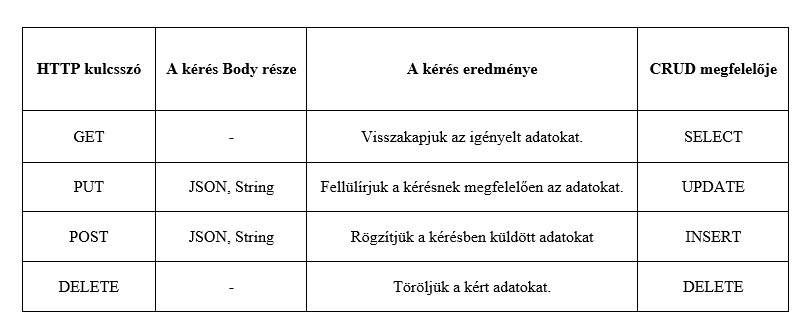
\includegraphics[scale=0.75]{kepek/rest.jpg}
\caption{RESTful szolgáltatások}
\label{fig:rest}
\end{figure}

\SubSection{Front-end}

A kliens oldal elkészítését \textit{Angular} keretrendszer segítségével oldottam meg \cite{4}. Azért esett a választásom erre a keretrendszerre, mert elég népszerű, jól dokumentált. Egy olyan környezetet biztosít, amivel a felmerülő problémák jelentős részét egyszerűen meg lehet oldani. Ez az előnye és a hátránya is, hiszen ha eltérünk az előirányzott fejlesztési elvektől -- más megoldást szeretnénk választani -- könnyen szélmalomharcot vívhatunk a keretrendszerrel. Ezek okán a legtöbb probléma felmerülése esetén könnyű megoldást találni az internet segítségével. A fejlesztéshez nem szükségszerű, de célszerűnek tünt \textit{Node.js}-t használnom \cite{17}.

Azért, hogy a felület megjelenése átvihető, egységes, rugalmasan átméretezhető legyen \textit{Bootstrap} modult használtam.

Szükség lesz \textit{Google Maps API}-ra, vagy egy másik térkép API-ra, ahol meg tudom jeleníteni a pozíciókat, hogy egyes helyszínek könnyebben behatárolhatóak legyenek.

\SubSection{Szerver-kliens architektúra}

Azért, hogy könnyebben átlátható legyen, készítettem az architektúráról egy általános ábrát (\ref{fig:architecture}. ábra).

Az asztali és a mobil alkalmazás az ábrán a teljesség kedvéért szerepel. A szakdolgozat keretein belül a böngészős kliens megtervezésére és megvalósítására került sor. A szerver oldalon a forráskódok és statikus állományok kezelésére ritkán lehet szükség, mivel a megjelenítendő adatok REST API-n keresztül jutnak el a böngészőbe. Szintén a teljesség kedvéért viszont célszerűnek tünt szerepeltetni őket az ábrán.

\begin{figure}[h!]
\centering
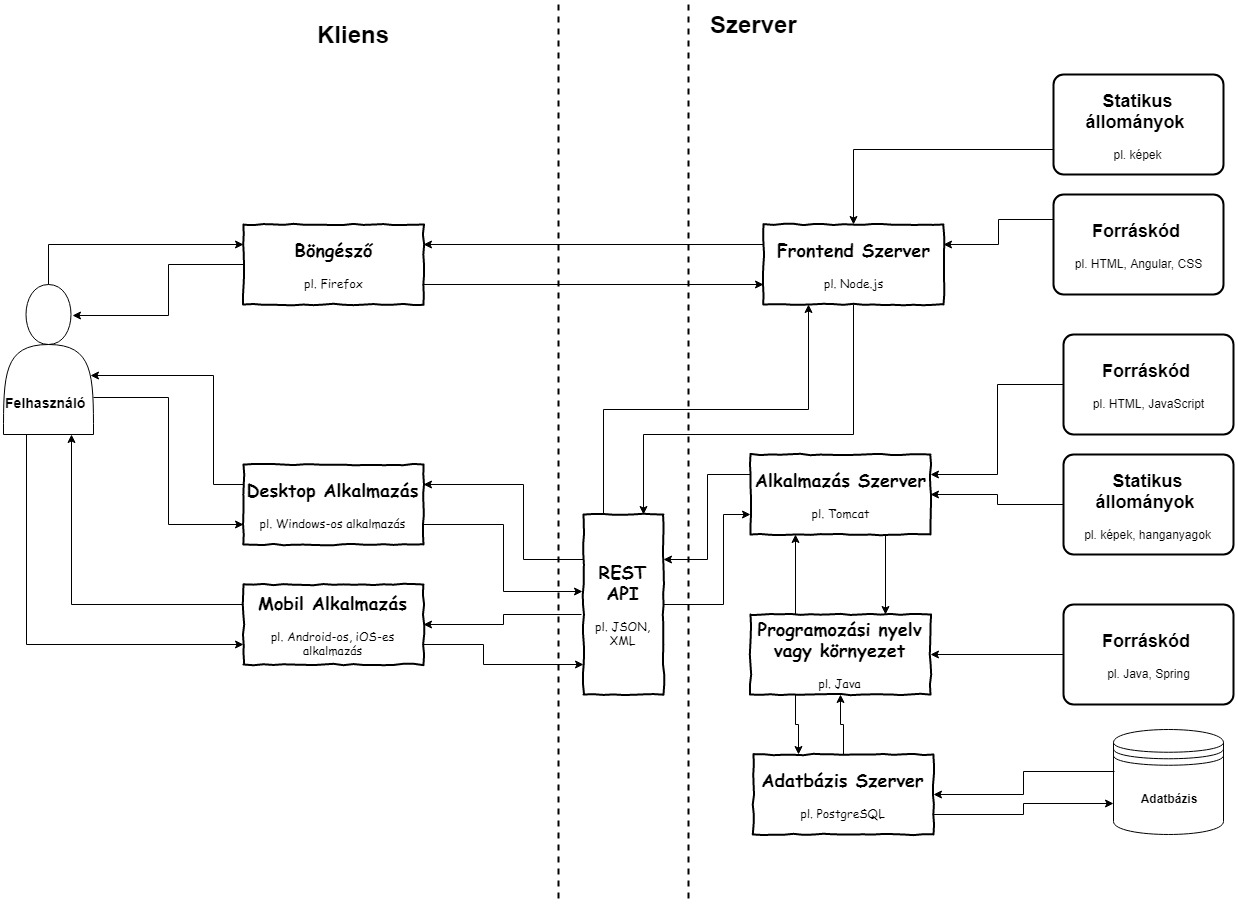
\includegraphics[scale=0.365]{kepek/architecture.jpg}
\caption{Szerver-kliens architektúra}
\label{fig:architecture}
\end{figure}

\SubSection{Fejlesztői környezetek}

A fejlesztéshez a \textit{JetBrains} termékeit fogom használni. A szerveroldali fejlesztéshez az \textit{InteliJ IDEA} nevű szoftvert, a front-end-hez pedig a \textit{WebStorm}-ot. Azért döntöttem mellettük, mert nagyon színvonalas eszközök, sokrétűen támogatják a fejlesztést.
 
A \textit{Postman} alkalmazást használom a minta kérések beküldéséhez, ezáltal a funkciók teszteléséhez szerver oldalon.

A \textit{JMeter} alkalmazást használom a stressztesztek elvégzéséhez és monitorozásához.

A szoftverek verziókövetését pedig a \textit{GitHub} segítségével végzem \cite{5}.

\Section{Az alkalmazás tervezése}

Az alkalmazás tervezésének és felépítésének egyik igen fontos lépése az adatbázis, annak sémáinak megtervezése. Ehhez a következőkben ER (\textit{Entity-Relationship}) modellt fogok használni, amely egy széles körben elterjedt és bevállt adatbázis tervezési módszer \cite{11}, \cite{12}, \cite{13}.

\SubSection{ER modell}

ER modellt használtam ahhoz, hogy szemléltessem az egyedek között fennálló relációkat és láthatóvá tegyem a megtervezett adatbázis architektúrát (\ref{fig:er}., \ref{fig:usEr}. ábra).

\begin{figure}[h!]
\centering
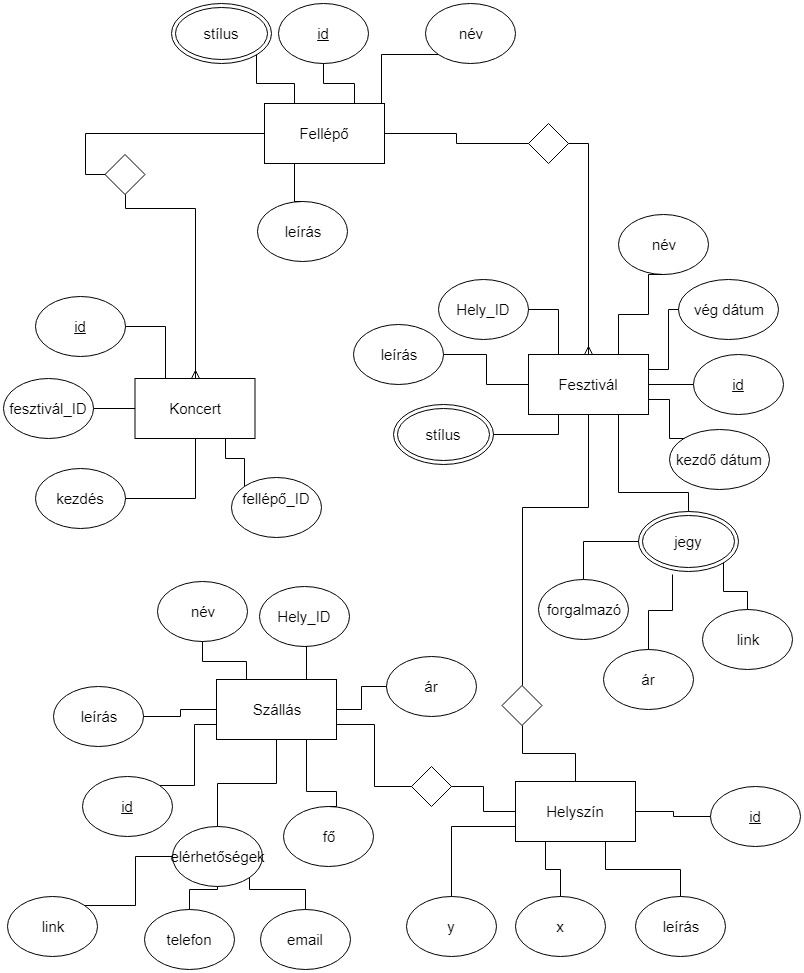
\includegraphics[scale=0.5]{kepek/er.jpg}
\caption{Az adatbázis ER diagramja}
\label{fig:er}
\end{figure}

\begin{figure}[h!]
\centering
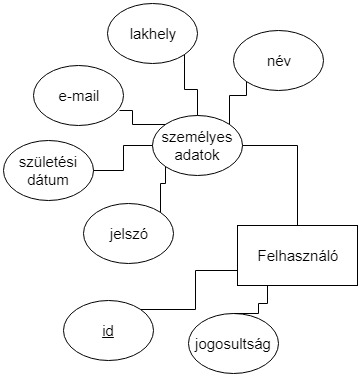
\includegraphics[scale=0.7]{kepek/userER.jpg}
\caption{Az adatbázis ER diagramja}
\label{fig:usEr}
\end{figure}

Lesz egy fellépő egyedünk, mivel alapvetően zenei fesztiválokban gondolkodunk, így ezek zenekarok, vagy zenészek lesznek elsősorban. Egy fellépő több stílusban is játszhat, hisz ha egy zenekar népzenét játszik, az nem zárja ki, hogy ezt ötvözzék rockzenei motívumokkal. Rengeteg előadó játszik több stílusban. A fellépőről tartunk számon egy rövid leírást. És elengedhetetlen, hogy az előadó nevét letároljuk. Tárolhatunk egy képet is az előadókról. Ezt egy központi mappában tesszük meg, viszont az előadóhoz tartozó fájl nevét a fellépő táblában is le kell tárolnunk. Az egyedi azonosítót pedig automatikusan generáltatjuk.

Egy fesztiválkereső alkalmazást készítünk, így nem meglepő, hogy lesz egy fesztivál nevű entitásunk is. Ez lesz a leginkább összetett. Minden fesztiválnak van egy neve, amely alapján a legkönnyebben azonosítják a rendszer felhasználói. Mivel egy ilyen esemény nem tart általában egész évben, ezért van egy kezdetét és végét jelző dátum. Erre a két időpontra azért is lesz szükségünk, hogy az érdeklő előre tudja  tervezni a programjait, és egyáltalán tudja, hogy nem ütközik-e valami más eseménnyel az általa kiválasztott fesztivál. Egy fesztiválnak is lehet több stílusa akár csak egy zenekarnak. Ahogy fentebb írtam, itt nem csak a stílusok férnek bele, hanem egyéb jelzők is. Az ID generálást itt is az adatbázisra bízzuk. A leírás részt azoknak az információknak tartjuk fent, amelyekre nem készítettük fel a rendszerünk, és a marketing szövegeknek is kiváló helyet biztosít. A jegy a fejlesztés első fázisában nem lesz bevezetve, így csak egy hyperlink-et tartalmaz majd a forgalmazó weboldalára és nem külön egyedként, hanem egy oszlopként reprezentálódik az adatbázisban. A fesztiválhoz is tartozik egy kép, itt is a nevét mentjük az adatbázisba, a képet pedig egy központi tároló mappába. 

A későbbi koncert táblában két idegen kulcs lesz megtalálható, mivel ez a tábla kapcsolja össze a fellépőt a fesztivállal, és ezáltal megtudjuk azt is, hogy milyen előadók vesznek részt az általunk preferált fesztiválon. Azt is megtudjuk nézni, hogy mikor kezdődik a számunkra érdekes előadás, mert egy kezdés nevű tulajdonságot is bevezettem. Lehetett volna tárolni azt is, hogy mikor van vége. Alapvetően ez csak egy kapcsoló tábla szerepet tölt be, így nem szerettem volna túlbonyolítani. (Feltételezem, hogy ha valakit érdekel egy program, akkor úgyis kivárja a végét.) Egyedi azonosítója ennek a táblának is lesz, amit itt is az adatbázisra bízhatunk.

A helyszínek adatainál címek pozícióit lehet tárolni. Erre azért lesz szükségünk, hogy le tudjuk tárolni, hogy pontosan hol lesz az esemény, vagy a szállás. Természetesen itt is lesz egyedi azonosító minden rekordunkhoz. Ha az $x$ és az $y$ koordinátát tároljuk, akkor rengeteg későbbi számítás egyszerűsödik. Van a Földnek egy egységes, minden tudományos intézmény által elfogadott geo koordináta rendszere. Ebben minden pozícióhoz tartozik egy hosszúsági és szélességi fok. Ezzel ki lehet váltani azt, hogy tárolni kelljen a várost, az utcát, a házszámot és az irányítószámot. Egy fesztivált szervezhetnek olyan helyre is, ahol ezek nincsenek is, akkor ahhoz egy másik struktúrát kellene bevezetni, amiben helyrajzi számot adunk át. És ha ezt a fesztivál szervező úgy kívánja megadni, hogy például az esemény egy adott csarnokban, vagy kulturális központban lesz, akkor megint egy újabb struktúra kerülne bevezetésre. Akkor viszont, ha csak a koordinátákat tároljuk, akkor ezeket valamilyen API-n keresztül, vagy előre mások által legyártott adatbázisból könnyen elérhetjük ezt egy koordináta rendszerbeli pont segítségével. A legismertebb Google nevű cég által készített térkép alkalmazást nézzük, ott az egyes koordinátákhoz, nem csak címeket, de akár éttermeket, boltokat, cégeket és minden egyebet tárolhatunk, sőt ezeket még értékelni is lehet. Egy leírást is tárolunk, itt meg lehet adni extra információkat, hol és hogyan közelíthető meg a megadott pont, illetve amíg nem integráljuk az alkalmazást egy API-hoz vagy egyéb elérhető lehetőségek közül addig magát a címet is itt tároljuk.

A szállásokat is tároljuk az adatbázisunkban. Lesz egy \textit{fő} nevű oszlopunk, amely azt tárolja, hogy a szállás hány személyt képes befogadni. Ez egy kisebb baráti társaság esetén lehet érdekes. Az ár tulajdonság egységárat tárol, tehát hogy mennyibe kerül egy éjszaka egy fő részére. Általában vannak egyedi konstrukciók, kedvezmények, de mivel mi nem foglalkozunk a foglalással, ezért csak irányárat mutatunk. Szolgáltatunk egy linket, ahol a foglalást el tudják végezni. Természetesen a szállás nevét is megadjuk. A címét az idegen kulcs segítségével könnyen megkaphatjuk. A leírásban minden egyebet tudunk rögzíteni. Az szállásadó elérhetőségeit is megadjuk az érdeklődök számára. A foglalási linken túl még egy telefonszámot és egy email címet is szolgáltat az alkalmazásunk.

Végül, de nem utolsósorban jönnek a felhasználóink, az alkalmazás regisztráció nélkül is teljes értékű alkalmazást nyújt egy keresni szándékozó felhasználó számára. A regisztrációra csak annak van szüksége, aki fel szeretne vinni az adatbázisba rekordokat. Itt több jogosultság is  felmerülhet.
\begin{itemize}
\item Fesztiválmenedzseri, aki a koncerteket, fesztiválokat viheti fel, ő felelős egy vagy több fesztivál menedzseléséért, a zenekarmenedzser, hasonló mint a fesztivál menedzser csak ő a fellépőkért felel.
\item Adminisztrátori, akinek mindenhez van jogosultsága ami elérhető az alkalmazásból.
\end{itemize}
Mi csak az adminisztrátori jogot fogjuk kiosztani, illetve az átlag felhasználót. A felhasználó személyes adatai közül az e-mail címét, nevét, születési dátumát és a lakhelyét, valamint a jelszavát tároljuk, amit valamilyen hasító algoritmuson lefuttathatunk előtte. Ez esetben is az adatbázisunk generálja az azonosítót.

Az egyedek között fent álló relációk a következőek:
\begin{itemize}
\item A fellépő egy-több kapcsolatban áll a koncerttel, hiszen egy fellépő több koncerten is felléphet, de egy koncerten csak egy fellépő szokott fellépni. Persze van rá példa, hogy van vendég előadó, de ezek az extrém esetek, amúgy is gyakran meglepetések.
\item A fesztivál és a koncert között is egy-több kapcsolat van. Egyértelműen megállapítható az, hogy egy koncert csak egy fesztiválon lehet megrendezve -- hasonló lehet máshol is, de egy fesztiválon több koncert is szokott lenni.
\item A fesztivál és a helyszín között egy-egy kapcsolat áll fenn, habár a helyszín akár lehet egy település is. Egy fesztiválhoz egy helyszín tartozhat, és egy helyszínen akár több fesztivál is megszervezhető, de a redundancia elhanyagolható volta miatt elég lesz számunkra az egy-egy kapcsolat. Egy fesztivál egy területen, nem pedig egy ponton helyezkedik el.
\item A helyszín és a szállás között egy-egy kapcsolat van, hiszen egy szálláshoz csak egy cím tartozhat.
\item A stílusok (vagy egyéb metaadatok) és az előadók között több-több kapcsolat van, de túl sok erőforrás pazarlásnak tartottam egy kapcsoló táblát bevezetni egy stílus miatt amiben semmi más nem tárolódik. Ezzel kapcsolatban több megoldást is számba vettem. Ezek közül például néhány: JSON vagy valamilyen NoSQL-ben eltárolom, és nem hozok létre a számára új táblát. Egy másik lehetőség egy saját struktúrának a bevezetése, például kettős keresztekkel elválasztva, és ez esetben sem lett volna új táblára szükségünk. Ezek a megoldások valamennyit gyorsíthattak is volna a megoldáson, de természetesen ezt tesztelés után lehetne eldönteni. Itt az egy-több kapcsolat megvalósításnál maradtam.
\item Az előzőhöz hasonlóan a fesztiválstílusok és a fesztivál között is ilyen a kapcsolat.
\end{itemize}

\SubSection{UML osztály diagram}

\begin{figure}
\centering
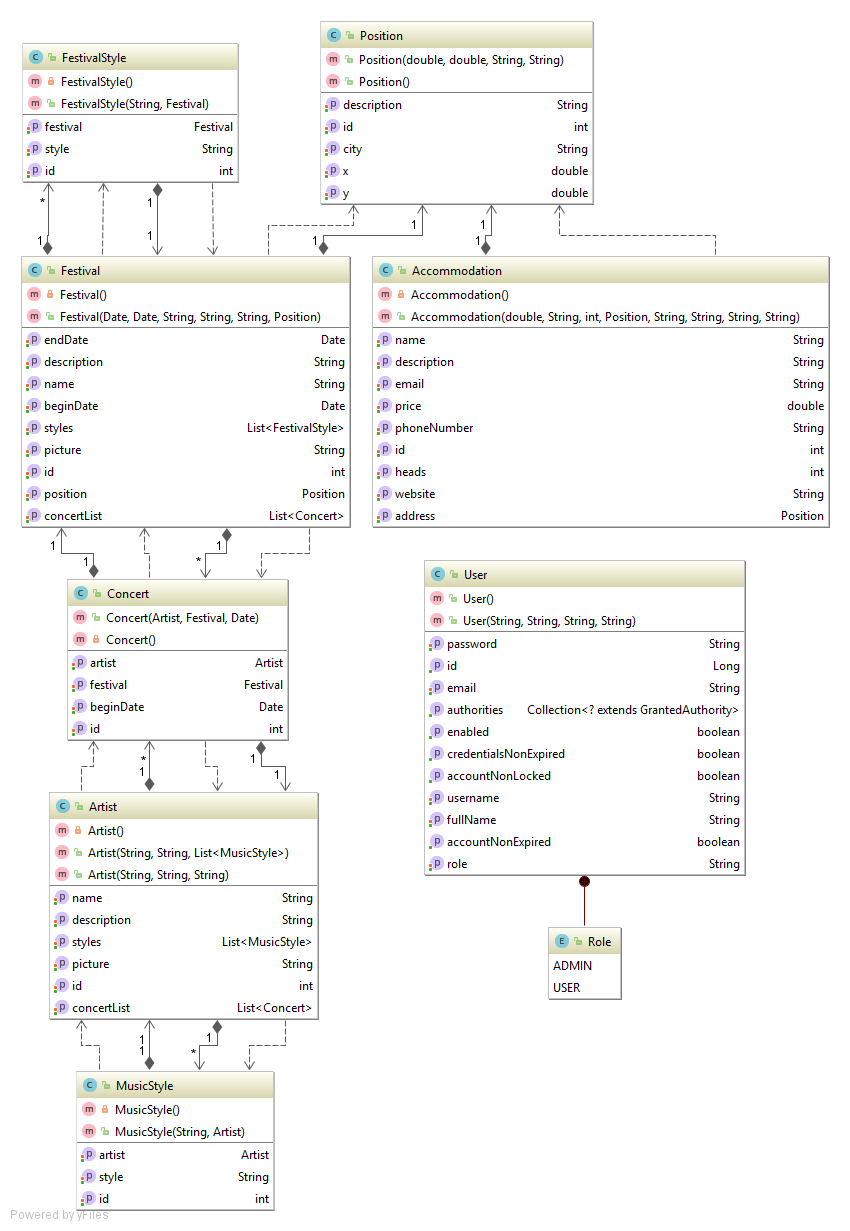
\includegraphics[scale=0.56]{kepek/uml.png}
\caption{A modell osztályok és kapcsolataik}
\label{fig:umlclass}
\end{figure}

Az ER segítségével megterveztem az adattárolási modellt és a \textit{bean}-eket. \Aref{fig:umlclass}. ábrán láthatjuk, ezek hogyan alakultak. Minden osztály tartalmaz egy privát, üres konstruktort és egy publikusat, amelyik minden adattagját tartalmazza, kivéve az azonosítót. Az \texttt{id} generálást a JPA-ra bízzuk, de mivel mindegyik \texttt{id}-m \texttt{Integer} típusú, így minden táblában az első elem az 1-es \texttt{id}-t fogja megkapni majd automatikusan 1-esével növekedni fog, tehát a második a ketteset kapja, és így tovább. Minden \textit{bean} osztályhoz fog tartozni egy \texttt{toString} metódus, és minden adattaghoz tartozik egy \textit{getter} és egy \textit{setter} metódus is. Ezek az ábrán nem szerepelnek (az átláthatóság érdekében), de definiálásra kerültek ezek is. Az adattagok természetesen privátok lesznek, míg az osztályok publikusak. A \texttt{User} táblához tartozik egy \texttt{Role} enumeráció, ami két értéket vehet fel: vagy \texttt{USER} vagy \texttt{ADMIN} lesz a rendszer által kezelt felhasználó.

\Section{Az alkalmazás rétegei}

\SubSection{Java csomagok struktúrája}

Az MVC (\textit{modell-nézet-vezérlő}) fejlesztési elvet követtem, de kibővítettem a \textit{Spring}-ben szokásos \textit{Service} és \textit{Repository} rétegekkel, és a \textit{View} réteget elhagytam, mert a megjelenítés majd a kliensben futó \textit{Angular} alkalmazás feladata lesz.

Nézzük meg, hogy az egyes rétegekben minek a tárolására lesz szükségünk.
\begin{itemize}
\item \textit{View}: A megjelenítésért felelős része az MVC modellnek, itt találhatóak a képek, a gombok, az űrlapok, ezzel találkozik a felhasználó, tehát maga a felhasználói felület. Én ezt a részét nem fogom használni a \textit{Spring}-nek.
\item \textit{Model}: A model, magyarul modell. Az adatok tárolásáért felelős része a kódnak, a perzisztenciáért is ez a rész felelős. Hasonló struktúrát kell követnie, mint az adatbázisnak. Én ezen a részen, mint már említettem a JPA technológiát fogom használni.
\item \textit{Contoller}: Itt találhatjuk meg az üzleti logikát. Itt történnek meg a számítások, innen jönnek a válaszok a felhasználó felé és innen mennek a kérések a modellhez. A Kontroller a kapocs a Modell és a Nézet között.
\item \textit{Service}: A \textit{Spring}-ben szokás bevezetni egy új réteget, ez lesz a Service, ennek segítségével ki fog válni az üzleti logika a \textit{Controller}-ből, és ezt a funkcióját átveszi a \textit{Service}. A \textit{Contoller} innentől forgalomirányítóként fog üzemelni.
\item \textit{Repository}: Bevezetésre kerül egy \textit{Repository} réteg is amely azért lesz felelős, hogy a \textit{Service} réteg részére előbányássza az igényelt adatok az adatbázisból, újat vigyen fel, módosítsa azokat vagy törölje, ha szükséges. 
Tehát az adatlekérdező és adatmanipulációs (CRUD) funkciókat valósítsa meg.
\end{itemize}

\SubSection{Angular csomagok struktúrája}

Az Angular-nál érdemes MVC szerű logikát használni, így a tervezésnél igyekeztem azt figyelembe venni. A kliens alkalmazás esetében a következő feladatokat látják el az adott rétegek.

\begin{itemize}
    \item \textit{Service}: Az alkalmazás ezen a rétegen keresztül kommunikál a szerver oldallal, itt jelentős üzleti logika nem jellemzi, mint a back-end oldalon. Főként a kéréseket szokás felépíteni ezen a szinten, tehát itt valósul meg a HTTP kommunikáció.
    \item \textit{Model}: A használt objektumok definícióját adjuk meg itt, és ezekre az objektumokra már le tudjuk képezni a kapott eredményeket.
    \item \textit{Component}:  Az \textit{Angular} komponensekbe szervezi a legfelső réteget, amelybe tartozik egy ts, egy css, és egy HTML fájl. A CSS és a HTML fájlok adják az oldal megjelenését tehát a \textit{View}-t. Az alkalmazás logkája \textit{TypeScript}-ben is implementálható, vagyis az, hogy az egyes bekövetkezett eseményekre az adott környezetben milyen válasz reakciót kell adni \cite{10}. A komponensek további komponenseket tartalmazhatnak, amelyek tudnak kommunikálni egymással.
\end{itemize}

\SubSection{A teljes struktúra bemutatása}

A projekt teljes szerkezetének áttekintéséhez nézzük meg \aref{fig:mvc}. ábrát! Ezt követően ennek az egyes részeit fejtem ki bővebben.

\begin{figure}[h!]
\centering
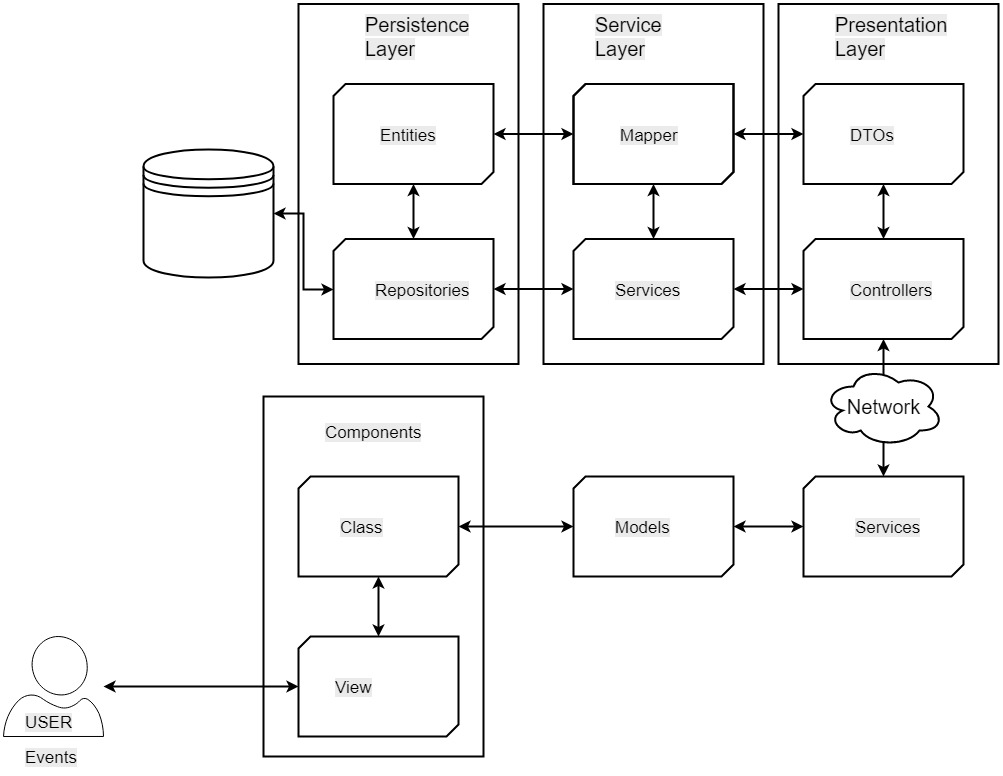
\includegraphics[scale=0.4]{kepek/mvc_arch.jpg}
\caption{Csomagok struktúrája}
\label{fig:mvc}
\end{figure}

Az ábrán megfigyelhető, hogy a repository osztályokon keresztül fér hozzá az adatbázishoz a rendszer. Természetesen az adatbázis eléréséhez, kell ismernie egy felhasználó név, jelszó párost, és egy elérési útvonalat a rendszernek, amelyet általában valamilyen környezeti változóban szokás megadni. A repository osztályokban fogjuk megadni az SQL lekérdezéseket, amelyeket gyakran ki sem kell írni, mert a keretrendszer az adatbázis struktúra ismeretében legenerálja a metódus neveket és megfogalmazza hozzá a lekérdezést, ha a \texttt{CRUDRepository}-t kiterjeszti az interfészünk. Természetesen ezek a nevek natív SQL-re konvertálódnak a lekérdezés alkalmával. Mivel ritkán fogunk bonyolultabb lekérdezéseket definiálni, így gyakran elegendő lesz, ha pedig bonyolultabb lekérdezést szeretnénk használni, akkor \texttt{@Query} paraméterként megadhatjuk, vagy natív SQL-ként vagy a JPQL lekérdező nyelv segítségével. A JPQL-t használom, mert ennek a szintaxisát jobban tudja kezelni az IntelliJ IDEA, és ad rá kódkiegészítést. A \textit{repository}-k lekérdezetnek olyan típusokkal, amelyek mező szinten definiáltak az adatbázisban vagy \textit{Entity} (\textit{bean}) típusokkal térhetnek vissza. A módosítás, törlés és új létrehozása is a \textit{bean}-ekre vonatkozik vagy annak egyes mezőire.

A \textit{service} rétegben foglalnak helyet a \textit{mapper} és a \textit{service} osztályok, interfészek. A szolgáltatásokat szokás interfészként megadni és létrehozni egy olyan osztályt, amelyik ezeket a szolgáltatásokat implementálja. A szolgáltatások metódusai a kontrolletről kapják a kéréseket és a \textit{repository}-hoz intézik a saját kéréseiket.  A \textit{service} osztályokban történik meg a beérkezett adatok feldolgozása és az elvégzendő műveleteket is itt hajtatjuk végre, majd a végrehajtott eredményeket letároljuk és/vagy kommunikáljuk a UI felé a kontroller segítségével. Általánosságban az is elmondható, hogy a repository felől entity-ket kezel míg a a controller felé \textit{Data Transfer Object}-eket (továbbiakban DTO). A \texttt{Mapper} osztályra azért lesz szükség, hogy a DTO osztályokat Bean-ekké és a Bean-eket DTO-ká alakítsa oda-vissza.

A kontrollerek azért felelősek, hogy figyeljék, hogy nem-e érkezik a kliens oldalról valamilyen kérés, és ha érkezett, akkor ezt kiszolgálják. Ez a modul állítja össze a kérésekre a válaszokat. Itt DTO formátumban fogadjuk az objektumokat, illetve ilyen formában is továbbítjuk őket a túloldalra. Mint már a service-nél említésre került, a controller a service-hez továbbítja a hálózaton kapott információkat a metódusaik meghívásával. A controller-nél minden metódus másik URI-n érkező kérésekre figyel, de ez triviális.

A túl oldalon is találkozunk a service-kel, itt azért felelnek, hogy a kérést intézzék a back-end felé és a visszakapott választ lekezeljék. A kapott értékek valamilyen modellre leképezhetőek, így definiálhatunk saját modelleket vagy használhatunk olyanokat is, amiket a keretrendszer definiál. Sajátokat fogok készíteni, amelyek a DTO-knak a tükörképei lesznek JSON formátumban definiálva, hiszen az Angular ezt az adatstruktúrát kezeli könnyedén. 

A komponensbe már modell formátumban érkeznek az adatok, a komponenstől is érkezhet modellt átadva a kérés a service felé, de a lekérdezéseknél ennél jóval kevesebb információ is elég. Ha az adatokon módosításokat végzünk, akkor természetesen minden releváns adatra szükségünk van és ilyenkor már modellt érdemes átadni a service metódusainak.
A komponens view része megjeleníti a böngésző segítségével a kapott információkat. A class része pedig szolgáltatja a megjelenítendő adatot, olyan formában amilyet a view igényel, illetve a kiváltott eseményeket kezeli, ha extra információra van szüksége, akkor azokat elkéri a service-ken keresztül.

Két típusú esemény van.
\begin{itemize}
\item Az egyik amelyiket a felhasználó vált ki azzal, hogy használja a rendszert. Ezek a nézeten keresztül érkeznek.
\item Vannak a felhasználótól független események is, amelyek akkor is kiváltódnak, ha a felhasználó nem nyúlt a rendszerhez. 
\end{itemize}

\SubSection{Példa egy kérés kiszolgálására}

Nézzünk meg egy példát a többrétegű alkalmazás működésére egészen a front-end-től az adatbázisig!
Tegyük fel, hogy egy űrlapot kitölt a felhasználó. Amennyiben minden mező értékét megfelelően megadta, és rákattintott a küldés gombra, akkor az meghívja az egyik service valamelyik metódusát. Ha nem sikerült megfelelően kitölteni, akkor jön egy figyelmeztetés a \textit{class}-tól, hogy mi a gond. Minimális mennyiségű alkalmazáslogikát a View is tárolhat. Előbb-utóbb, ha sikerül mindent megfelelően kitöltenie a felhasználónak, akkor már a service réteghez is eljut, ahol egy HTTP kérést intéz a szerverhez. Itt az interfész érzékeli, hogy jött valamilyen kérés és megpróbálja leképezni a kontrollerekre, ha nem sikerül akkor visszautasítja, ha viszont talál olyat amelyikre illeszkedik, akkor a gondjaira bízza a kapott információkat. Természetesen ettől még megtagadhatja a kiszolgálást, ha olyan tartományból jön a kérés, vagy nem azonosította magát a kérelmező fél és ezt a rendszer igényli. A kontroller tovább hívja a service réteget és átadja neki a DTO objektumot paraméterként. Itt pedig a repository rétegnek hívjuk meg a mentés metódusát. Persze előtte le kell képezni a DTO objektumot \textit{bean}-né. Ezt megtehetjük \texttt{Mapper} osztály segítségével vagy kézzel is. Struktúrától függően ki is hagyhatjuk a DTO objektumokat és ilyenkor már a kontroller réteg \textit{bean}-t vesz át. A visszatérési értéket pedig a hívási láncon visszafele elindulva eljuttatjuk a front-end-nek, és ha minden rendben ment, akkor ezt jelezzük a felhasználó számára, ha nem akkor informáljuk a hiba okáról.
 
\Section{Szerepkörök és jogosultságaik}

A használati eset (\textit{Use Case}) diagramot arra használom, hogy megmutassam azt, hogy az egyes jogosultsági szinttel rendelkező felhasználók az alkalmazás milyen funkcióihoz férhetnek hozzá. Ahogy azt már említettem, minden, a rendszerbe belépett felhasználó adminisztrátor (\textit{admin}) lesz, külön privilegizált jogkört a felhasználóknak (\textit{user}-eknek) nem hozunk létre. Az alkalmazás tehát egy központosított fesztiválszervező alkalmazásnak tekinthető, melyben a \textit{User} jogosultsági kör tulajdonképpen a neve alapján arra utal, hogy a rendszer felhasználói, viszont jellemzően a weboldal látogatójának tekinthetjük. A \ref{fig:useCase}. ábrán megtekinthető, hogy az adminisztrátor adatmanipulációs műveleteket is végezhet, addig a felhasználó csak megtekinthet mindent. Bejelentkezni csak az adminisztrátor tud, hisz neki van fiókja. Ebből következik, hogy kijelentkezni is csak ő tud. Regisztrálni a felhasználó is tud, ha ezt megteszi, jóváhagyást követően adminisztrátorira bővül a jogköre.

\begin{figure}
\centering
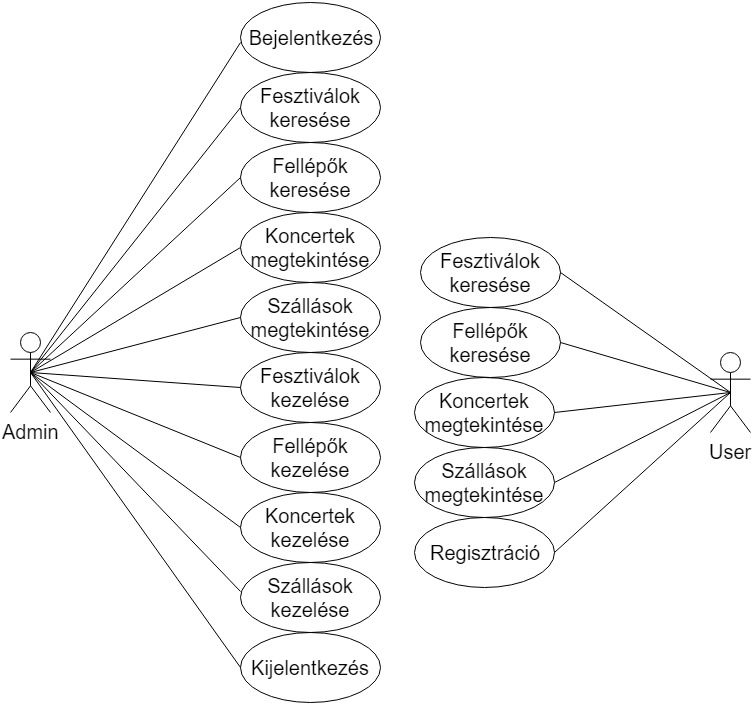
\includegraphics[scale=0.55]{kepek/use_case.jpg}
\caption{Az adminisztrátori és a felhasználói szerepkörökhöz tartozó funkciók}
\label{fig:useCase}
\end{figure}

\Section{Konkrét funkciók}

\SubSection{Lekérdezések}

A következő pontok bemutatják, hogy egy ilyen rendszerben milyen lekérdezésekre lehet szükség, és ezt milyen formában kezeli a rendszer.

\begin{itemize}
\item \textit{Az összes fesztivált visszaadó funkció}, amely mindezt a kezdés időpontja szerint adja vissza, illetve amelyik fesztivál már véget ért azt már nincs értelme visszaadni a felhasználónak. Ez az alapértelmezett, ha a fesztiválok menüpontra kattintunk. A megvalósítása egy egyszerű lekérdezés eredménye lesz az adatbázisból. Mint minden lekérdezés, ez is az egész hívási láncon végig fog menni, amit a korábbi példában említettem. Ahol ez megkerülhető azt külön jelezni fogom.
 
\item \textit{Egy konkrét fesztivál visszaadása}. Ez akkor aktiválódik, ha egy fesztivált kattintással kiválasztunk a felületen, és ezáltal több információt szeretnénk róla megtudni. Ez kettő vagy három hívást fog generálni. Megtehetjük azt, hogy átadjuk a fesztivál modelljét a listából a fesztiválrészletek weboldalnak, vagy az azonosítója alapján lekérdezzük újra. A lekérdezés mellett döntöttem, mert a többi lekérdezést így-is úgy-is végre kell hajtani és azokat is \texttt{id} alapján fogjuk megtenni. Az egyik ilyen kérés ez esetben a fesztivál közelében lévő szállások lekérdezése, a másik pedig a fesztiválhoz tartozó koncertek listája.   

\item \textit{Fesztivál koordinátáitól 10 km távolságon belülre eső szállások}. Akár lehetne megadott távolság szerinti keresés, de a szállás keresést nem szeretném a felhasználóra bízni. A fesztivál kiválasztásakor ajánl a rendszer a fesztiválhoz közeli szállásokat, amikor az előző pontban meg szeretne tudni több információt egy fesztiválról. A későbbiekben akár ez megvalósulhat önálló funkcióként is, ahol megadott koordinátától, megadott távolságra lévő szállásokat tudunk megkeresni. Ez esetben majd a megadott koordináta lehet a fesztivál, és a felhasználó meg kiválaszthatja majd, hogy milyen távolságon belül szeretne találni, de egyenlőre rögzített távolságérték lesz megadva.

\item \textit{Koncertek fesztivál alapján.} Ez a másik lekérdezés lesz, amikor egy általunk kiválasztott fesztivál programját betöltöttük. A fesztivál azonosítója alapján elkérjük a szerver oldalról azokat a koncerteket, amelyek a megadott fesztiválhoz kapcsolódnak, és kijelezzük a felhasználó számára a koncert kezdés idejét és fellépő nevét. Itt, ha a fellépőre kattint, akkor a fellépőről is megtudhat információkat. A későbbiekben valamilyen rendezési elv is bekerülhetne. Jelenleg csak egy listaként kezeli a rendszer. A későbbiekben lehetne napokra bontani, vagy színpad szerint csoportosítani, ehhez viszont az adatstruktúrába egy színpad elemnek is be kell majd kerülnie. Ez a tervezés előző fázisaiból kimaradt.

\item \textit{Fesztiválok névrészlet alapján.}  Ez azoknak kedvez, akik már tudják mit keresnek, és az esemény programját szeretnék megtekinteni. Ez elég lehet csak a front-end-en kezelni egy hozzárendeléssel, azokra szűrve, amely fesztiválok nevében megtalálható a megadott névrészlet. Ilyen esetben nem kell gombot nyomni a felületen, hanem elég, ha csak azt figyeljük, hogy történt-e változás a bemeneten, és ha igen akkor újra map-peljük a tömböt.

\item \textit{Kiválasztott stílus alapján} megkapjuk azon fesztiválok listáját, amelyek a kategória alá tartoznak. Ez kétféleképpen fog megvalósulni. Az egyik a \textit{hashtag}-re kattintva, leszűri azokat a fesztiválokat, ahol megtalálható a megadott stílus. Ekkor nem muszáj elkérni a back-end-től a kellő információkat, elegendő az adott feltételek szerint megcsinálni a leképzést. A másik a részletes keresés esetén, ez majd a következő pontban fejtem ki.

\item \textit{Komplex keresés.} Ez alatt több keresési kritérium szerinti keresést értünk. Az egyes lehetőségeket alább pontokba szedve részletezem.
\begin{itemize}
\item Meg lehet keresni település alapján, illetve településtől való távolság alapján. Ez úgy fog megvalósulni, ha a rendszer felhasználója megadja a fesztiválkereső modulban a települést, akkor a térkép API-tól elkérjük a hely koordinátáit, és majd azokat küldöm be, ha a felhasználó ad meg távolságot is a pozíciótól akkor a távolságot is itt küldheti át. Ezzel kapcsolatban felmerül egy kérdés, hogy hogyan lesz a koordinátákból km érték és fordítva? Szerencsére nem én vagyok az első, aki ezt a kérdést felteszi, így az internet segítségével gyorsan rátaláltam a \textit{Haversine} formulára. A módszernek az esetünkben van egy kis hibája, hiszen gömbbel számol, de mint tudjuk a föld geoid. Ez egy Magyarország méretű és természeti adottságú ország esetén jelentős torzulást nem okoz. A formulába behelyettesítve a két $x$ és a két $y$ koordinátát, ezzel megkapjuk a távolságukat kilométerben. Amennyiben az kisebb, mint a megadott távolság, akkor megfelel számunkra, ha nem akkor sajnos nem. Mivel egy település koordináták halmaza, így akkor is alkalmaznunk kell a Haversine algoritmust, ha nem adott meg a felhasználó paramétert ilyen esetben 5 km alatti eredményekre szűrünk. 

\item Fesztiválokat kereshetünk két dátum közötti intervallumban. Ha a felhasználó az egyiket, vagy mindkettőt üresen hagyja, arra is fel készítjük a rendszert. Mindkettő üresen hagyásának esetén akkor a lekérdezés időpontjában még véget nem ért fesztiválokat adjuk vissza. Ha a felső érték üres és az alsó érték van megadva, akkor a keresés időpontjában még véget nem ért fesztiváloktól a megadott időponting elkezdődötteket adjuk vissza. Ha az felső érték van megadva, akkor a megadott időpontkor már elkezdődötteket adjuk vissza. Ha mind kettő meg van adva, akkor az előző két keresésnek a metszetét adjuk vissza.

\item Stílus alapú keresés a fesztiválhoz. A jegyeket nem valósítjuk meg és úgy döntöttem, hogy a stílusoknál jelenítem meg. A \#free paramétert vezettem be a stílusoknál erre az esetre. Innentől ez egy stílus lesz és ezt is a stílusoknál kezelem. Emiatt megint lesz 4 esetünk. Az első, nem pipáljuk be a jelölőnégyzetben, hogy ingyenes, és nem adunk meg semmilyen stílust, ez esetben a keresést nem érintik ezek a paraméterek. A második, megadjuk hogy ingyenes, ilyenkor azokat a fesztiválokat szelektáljuk le amihez tartozik egy free stílusú címke(hashtag). A harmadik eset, ha csak stílus van megadva. Ugyan az történik mint az előző esetben, csak nem \textit{free}-vel küldjük be a kérést. Amikor mind kettő megvan adva, akkor pedig a stílussal küldjük be a kérést, és a visszakapott listából még leszűrjük azokat amelynek van free stílusa is és csak azokat adjuk át a felület számára.
\item Az itt felsoroltak kombinációira is fel kell majd készítenünk a programunkat, a felsoroltak alapján méltán kapta a komplex keresés nevet ez a pont.
\end{itemize}

\item \textit{Az összes fellépő visszaadása.} A fellépők menüpontra kattintva elkérjük az adatbázisban található összes fellépőt, és kilistázzuk ezeket. Hasonló, mint a fesztiváloknál, csak itt nem kell annyi speciális esetre figyelnünk.

\item \textit{Fellépők visszaadása névrészlet alapján és/vagy stílus részlet alapján.} Ugyanúgy fog működni, mint a fesztiváloknál a név részlet szerinti keresés, csak itt még egy metódus fog figyelni, hogy nem-e történt változás. 

\item \textit{Az összes olyan fellépő visszaadása amelyiknek a stílusa megegyezik a lekért stílussal.} Ez akkor következik be, ha \textit{hashtag}-re kattint a felhasználó, ilyenkor lekérdezzük azokat a stílusokat, amelyek értéke megegyezik a kérttel, mivel a JPA össze is kapcsolja a fellépővel, így már csak annyi a dolgunk, hogy visszaadjuk a stílusokhoz tartozó fellépőket.

\item \textit{Fellépő részletei}, a fellépő összes részlete elérhetővé válik számunkra. Ez ugyan azt a struktúrát követi, mint a fesztiváloknál volt, csak ide nem tartoznak szállások, viszont a koncerteket itt is elérhetjük.

\item \textit{Koncertek fellépő alapján}, itt a pontos időpont is kiderül, hogy mikor lesz a fellépés, egy egyszerű szelektálás a fellépő id-ja alapján. Ez akkor hívódik meg amikor a fellépő részleteit kívánjuk betölteni.

\item \textit{Összes stílust visszaadó funkció}, amely értékkészletből könnyebben tud választani, ha esetleg nem jutna eszébe, vagy nem gondolna az esetleges kategóriákra. Itt le kell kérdezni az összes stílust és egy szűrést kell végezni, hogy mindegyik csak egyszer szerepeljen a listába. Ez a keresés illetve az új felvitele esetén jöhet jól.
\end{itemize}

\SubSection{Új elemek hozzáadása}

A következő pontokban azon módosító funkciókat vesszük sorba, amelyek új elem hozzáadásával járnak.

\begin{itemize}
\item \textit{Szállás felvitele pozíciójával együtt.} Itt oda kell figyelni arra, hogy minden olyan mezőt kitöltsön a feltöltő ami a szállás szempontjából releváns, a back-end oldalon pedig fontos a hozzátartozó pozíciót is lementeni, nem elég csak a szállást.

\item \textit{Fesztivál felvitele pozíciójával és stílusaival együtt.} Miden releváns adatra szükségünk lesz, egyes értékeket validáni is érdemes, ilyen lehet a koordináták értéke. Hiszen ez 180-tól -180-ig terjedhet, vagy a fesztivál kezdete ne legyen később, mint a vége. Itt a stílusok lementésére is oda kell figyelni, a pozícióján kívül.

\item \textit{Zenekar felvitele a stílusaival együtt.} A stílusok lementésére oda kell figyelni és arra, hogy a releváns adatokat bekérjük, a felviteleknél a JPA-ra bízzuk az id generálást, mint már azt a fejezetben említettem.

\item \textit{Kép felvitele.} A front-end-en elkészül egy képfelvivő modul és ezt több helyen is el fogom helyezni. A fesztiváloknál és a fellépőknél mindenképpen, a front-end-en a képfeltöltő service osztályának a feltöltés metódusa mindig azt a path-t hívja meg amit paraméterben megkap, tehát ha a fesztiválét akkor a fesztivál kontrollerének megfelelő metódusát fogja meghívni. A path-nak része az id. A túloldalon aszerint mentjük le ahonnan érkezett. Először módosítjuk a képnevét, valami randomizált dolgot hozzá kell fűzni, hogy ugyanolyan nevű képből akár több is felkerülhessen. Le kell kérdezni id szerint azt az objektumot aminek megkaptuk az id-ját és típusát és annak módosítani a kép adattagját a kép nevére, a képet pedig egy közös mappába mentjük el, ahonnan a neve alapján már könnyen kinyerhető, ami ilyenkor már az egyedi azonosítója lesz.

\item \textit{Koncert felvitele}, ami valójában egy fellépő és egy fesztivál összekapcsolása. Itt az összes fesztivált és fellépőt bekérem egy listában, és a listából kiválaszthatja az admin, hogy melyik fesztiválhoz, melyik koncertet szeretné felvinni. és még egy kezdési időpontot kell kiválasztania és már mentheti is.

\item \textit{Új, további stílusok hozzáadása zenekarhoz.} A módosítás menüben tudja majd felvinni illetve lecserélni, törölni a stílusokat.

\item \textit{Felhasználó regisztrációja.} A kötelező adatok megadása után lehet regisztrálni a rendszerben, arra oda kell figyelni, hogy a két jelszónak meg kell egyeznie, egyébként nem rögzíthetjük az adatbázisban, mert elképzelhető, hogy az egyiket elgépelte.
\end{itemize}

\SubSection{Módosítások}

Azon műveleteket vesszük sorba, amelyek már meglévő adatok módosításával járnak.

\begin{itemize}

\item \textit{Stílusok módosítása} a fesztivállal vagy a fellépővel együtt történik.

\item \textit{Kép cseréje}, új fájl feltöltésével történik meg, ilyenkor az adatbázisban az új kép nevére jön létre referencia.

\item \textit{Fesztivál módosítása}, ezen belül meghívandó a helyszín módosítása és itt hajtható végre a stílusok törlése, módosítása, vagy új felvitele. A beküldött adatokat lecseréljük a megadott id alapján, természetesen az id nem változtatható.

\item \textit{Zenekar módosítása.} A fesztivál törléséhez hasonlóan lehet a stílussal  kapcsolatos módosításokat elérni a felületen, és az adatok cseréje, ritkán van rá szükség.

\item \textit{Koncert módosítása}, jelenleg nem releváns.

\item \textit{Szállás módosítása}, jelenleg nem releváns. Ez nem kerül megvalósításra.
\end{itemize}

\SubSection{Elemek törlése}

Az utolsó jellegzetes művelet a törlés. Ezekre az alábbi formában lehet szükség a fesztiválszervező alkalmazás esetében.

\begin{itemize}
\item \textit{Stílusok törlése}. A fesztiválok és fellépők módosításánál érhető el ez a funkció.

\item \textit{Kép törlése}. Akkor törlődik a régi kép, ha újat rakunk fel. Pontosabban lecserélődik, mert a képet nem törlöm, csak a referencia szűnik meg ami rá mutat.

\item \textit{Fesztivál törlése.} Itt figyelni kell arra, hogy a törlés előtt fel kell szabadítani minden olyan erőforrást ami függ tőle. Tehát törölni kell a koncertjeit, stílusait és a fesztiválhelyszínt is.
\item \textit{Fellépő törlése.} Nem jellemző, de ha mégis szükség lenne rá, akkor a stílusait is törölni kell.
\item \textit{Szállás törlése}. Itt is figyelni kell, hogy a hozzátartozó helyszínt is törölni kell vele együtt.
\item \textit{Véget ért koncertek}. Amelyik fesztivál és koncert elmúlt, tehát a befejezés dátumán már az aktuális naptári idő  túlhaladt, azt archiválni kell. Erre a funkcióra elég egy trigger-t írni. Archiválás megvalósítása megoldható úgy, hogy átmozgatjuk egy másik táblába, vagy egy új változó bevezetésével, és azt hogy elérhető-e elég igazról hamisra állítani. Esetleg a mindent vissza adó függvény csak azt adja vissza amelynek a befejező dátuma nagyobb mint az aktuális dátum.
\end{itemize}

\Section{Hibalehetőségek és kezelésük}

A következő szakaszokban néhány jellemző hibajelenséget vizsgálunk meg.

\SubSection{Adatbázishoz kapcsolódás}

Adatbázis műveletek esetén előfordulhat, hogy valamilyen okból nem érhető el az adatbázis, ilyenkor \texttt{SQLException} váltódik ki az egyes adatbázis műveletek esetén. Nekünk erre azért nem kell jelenleg még nem kell készülnünk, mert az adatbázisunk egy in-memory h2, ez a szoftverrel indul és áll le és külön hálózat sem kell hozzá, hogy elérjük. Ha valódi adatbázisra cseréljük, akkor kivételkezelést kell minden olyan kódrészhez írni, amelyik az adatbázissal interakcióba lép.

\SubSection{Adatbázisból \texttt{null} értékkel való lekérdezés}

Az adatbázisból nem szabad \texttt{null} értékkel lekérdezni. Ezt helyes kódszervezéssel ki tudjuk kerülni. A \textit{Spring Security} segítségével be lehet állítani úgy, hogy a rendszert csak megadott IP címekről érkező kérések tudnak módosítani back-end API-n keresztül.

\SubSection{Rossz adattípus érkezik}

A felhasználói felületről új adat felvitelénél rosszul kitöltött adatok esetén előfordulhatna az, hogy például numerikus adat helyett egy string érkezik, és azt sajnos nem tudja kezelni a keretrendszer. Ilyen esetben \texttt{NumberFormatException} keletkezik, ha a felhasználói felületen minden beviteli mezőt szigorúan validálunk, akkor ilyen nem fordulhat elő. Esetleg érdemes lehet kivételkezelést is használni a backend oldalon, ahol ez bekövetkezhet. 

